\subsection{Standardization Efforts}
Standardization of technologies have huge implications on their usage. In a post from the IETF they say "standards form the fundamental building blocks for product development by establishing consistent protocols that can be universally understood and adopted". The Internet is build on open standards like HTTP, TCP, IP, HTML, URL and MAC which enabled it to thrive. It gives developers technical security and provides them an abstraction layer which they can develop against. Because of the novelty of running Kubernetes on the edge there is still considerable effort to standardize the edge components and communication protocols.\\[5mm]
% Standardization efforts IETF, CoAP (hadnled by IETF), CNCF edge working group, protobuf and grpc
{\textbf{\textit{Constrained Application Protocol}}}\\
Constrained Application Protocol (CoAP) is a "specialized web transfer protocol for use with constrained nodes and constrained networks"\cite{CoAPCon75:online} and is standardized under the IETF id 7252\cite{RFC7252CoAPIETF}. It is an application layer protocol similar to HTTP\textbackslash1 (or 2)  but utilizes UDP instead of TCP as transport layer protocol. The primary reason for this design choice is to keep the IP overhead as low as possible. It behaves similar to HTTP\textbackslash1 (or 2) in that it utilizes the REST model with a subset of its methods, e.g. \textit{GET, PUT, POST, DELETE} etc. Additionally, it offers caching of responses and proxying between CoAP and HTTP. It implements a stateful connection in the application layer rather than in transport layer and uses DTLS which works over unreliable data transfer connections. This is more efficient and does not require the typical three way handshake a TCP connection would require.

Compared to other IoT protocols CoAP is easier to understand as it uses the same concepts of the Internet stack. \Cref{fig:mqttVsCoap} shows side by side the architecture of MQTT and CoAP. Both are optimized for the IoT space and can do machine to machine (m2m), but their architecture is fundamentally different.
\begin{figure}[h!]
    \centering
    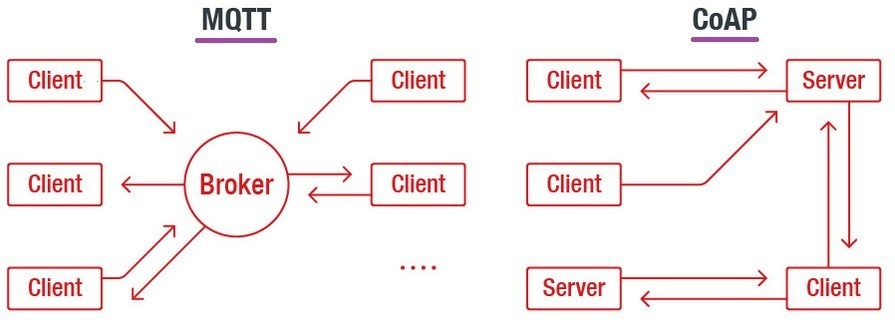
\includegraphics[scale=0.45]{figures/mqtt-vs-coap.jpg}
    \caption{MQTT and CoAP Architecture side by side\cite{COAPvsMQTT27:online}.}
    \label{fig:mqttVsCoap}
\end{figure}
MQTT is based on the publish-subscribe massaging pattern which relies on a central entity, called broker, to enable communication between multiple nodes. Researches compared the two standards and found "MQTT messages experienced lower delays than CoAP for lower packet loss and higher delays than CoAP for higher packet loss"\cite{MQTTvsCoAPAnalysisIEEE}. They also found that the message overhead for small messages is significantly lower at 25\% or less for CoAP compared to MQTT for reliable message transmission. But MQTT is by default synchronized across the cluster while CoAP is not. To combat this the standard was extended by the "observable" method in 2015\cite{RFC7641observableCoAP}. This makes it possible for a client to subscribe to a server resource and keep it updated by the server. and is very close to the publish-subscribe massaging pattern from MQTT.\\[5mm]
{\textbf{\textit{Protocol Buffers}}}\\
Protocol Buffers (Protobuf) are not yet standardized and only have an expired proposal under the IETF\cite{rfernando-protocol-buffers-00}. However, they are widely used for data serialization. Compared to JSON which is an IETF standard, protobufs are sent as binaries and thus not human readable. The protobuf message structure needs to be defined on the client and server side and represents an explicit contract of information exchange between the two. When an entity sends data as protobuf, the compiler appends an indicator of which field a binary string belongs to. Whereas in JSON both the identifier and the value are transmitted, in protobufs the identifier is a position in the data structure and put in front of its value.
When researches compared the message sizes of JSON to protobufs they found huge differences between the two, shown in \cref{fig:jsonVsProtobufs}.
\begin{figure}[H]
    \centering
    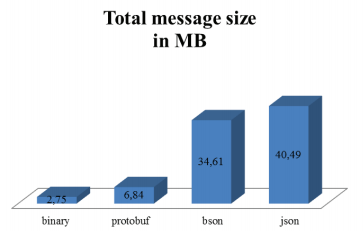
\includegraphics[scale=0.6]{figures/jsonVsProtobufs.png}
    \caption{Memory Consumption of different Serialization Protocols\cite{jsonVsProtobufs}.}
    \label{fig:jsonVsProtobufs}
\end{figure}
The researches conclude "the Protocol Buffers are a serious candidate for standardized way of communication in field of Internet of Things"\cite{jsonVsProtobufs}.\\[5mm]
{{\textbf{\textit{Kubernetes IoT Edge working group}}}}\\
The Kubernetes IoT Edge working group\cite{IntroducingDejanBosanac:KubernetesIoTEdgeWorkingGroup} was introduced in mid 2018 and is a platform for companies to develop open edge standards in connection with Kubernetes. The Cloud Native Computing Foundry (CNCF) under which Kubernetes resides "saw more and more developers trying to use Kubernetes outside typical data center deployments"\cite{IntroducingDejanBosanac:KubernetesIoTEdgeWorkingGroup}, especially on the edge. It wants to bring the cloud-native best practices and tools to the edge. The projects proposed in the working group are not all based on Kubernetes but are supposed to seamlessly integrate into its existing workflow. The group has identified many problem areas Kubernetes is not yet ready to deal with. This includes trusting of unconnected hardware, trusting of connected devices, secure operating system, network concerns and integrity of software. These areas are immensely important and an open solution would have a huge impact on the edge industry, just as Kubernetes had for the cloud industry.



